\documentclass[../Main.tex]{subfiles}
\begin{document}

\section{Introduction problems}

\subsection{Problem statement}

This is a website containing a large amount of information about houses and rooms that the owners do not currently need and want to rent out.
Visitors to the website can use search functions based on location, such as by city, district, or by specific address, like the house number on a particular street.
They can also search by rental price and the amenities of the houses or rooms available for rent.
The website provides detailed information about the houses or rooms available for rent, including the address and contact phone number for the landlord.

Instead of visiting each place to see rental properties, users only need an internet-connected device to access the website and search for the rental information they need, then contact the landlord.
The website also offers a real-time chat feature for users to conveniently exchange information.

\subsection{Purpose of this system}

\begin{itemize}
    \item User Interface: Design an intuitive interface that is easy to navigate and visually appealing.
    \item Basic Functionality: Implement essential features such as search functionality for finding rental information and an upload feature for landlords to post room details.
    \item Optimized Performance: Ensure the website is highly responsive by optimizing response times and loading speeds.
    \item Cost Efficiency: Minimize costs and distances for both landlords and tenants by efficiently connecting them through the platform.
    \item Admin Management: Provide an easy-to-use admin interface for managing room information and user interactions.
    \item Accurate Data Management: Ensure precise storage and retrieval of data to provide reliable information to users.
\end{itemize}

\section{Requirements Specification}

\subsection{Software Requirements Specification}

This document specifies the detailed requirements for a room rental web application, catering to administrators and customers.
The application aims to facilitate efficient room management and rental transactions.

\begin{table}[ht!]
    \caption{User Roles and Descriptions}
    \label{table:roles}
    \centering
    \begin{tblr}{|c|X|}
        \hline
        Role 1    & Descriptions \\
        \hline
        Admin     &
        Room and Pricing Management: Add, edit, and delete room types and pricing tiers.

        User Management: Manage user accounts, including CRUD operations.

        Confirmation of Uploaded Rooms: Review and approve rooms uploaded by landlords.

        Statistical Analysis: Generate reports on revenue, number of rooms in each region.
        \\
        \hline
        Customers &
        Search Functionality: Search for rooms based on room type, price range, area, etc.

        Registration and Login: Create an account and securely log in.

        Account Funding via Momo: Deposit funds into the account via Momo wallet to post more room listings.
        \\
        \hline
    \end{tblr}
\end{table}

\subsection{Functional Requirements Specification}

\subsubsection{Main Features of the Website}

Storage of Room Rental Information:
\begin{itemize}
    \item Store details about houses and rooms available for rent, such as location, address, rental price, and contact information for landlords.
    \item Ensure structured data storage for efficient and quick search functionality.
\end{itemize}
Attractive and User-Friendly Interface:
\begin{itemize}
    \item Design an appealing and user-friendly interface accessible to all user types.
\end{itemize}
Flexible Search Functionality:
\begin{itemize}
    \item Implement versatile search capabilities allowing users to quickly find rental information based on location, price range, and other relevant criteria.
\end{itemize}

\subsubsection{Users}

User Registration and Authentication:
\begin{itemize}
    \item Users can register for an account on the website.
          Upon successful registration, a confirmation code will be sent to the registered email address for verification.
    \item After successful verification, users can log in to the system using their credentials.
\end{itemize}

Flexible Room Search:
\begin{itemize}
    \item Users can search for rental properties based on various criteria such as price, location (address or region), room type, and area size.
\end{itemize}

Room Upload and Fee:
\begin{itemize}
    \item Users with authenticated accounts can upload room rental information.
          Each room upload will incur a fee of 10000 VND per submission.
\end{itemize}

Management of Uploaded Room Information:
\begin{itemize}
    \item Logged-in users can manage the details of rooms they have uploaded, including editing or deleting listings as needed.
\end{itemize}

\subsubsection{Admin}

User Management:
\begin{itemize}
    \item Admin can manage user accounts, including viewing user details and account statuses.
    \item Admin has the authority to suspend or deactivate user accounts if suspicious activities are detected.
\end{itemize}

Room Category Management:
\begin{itemize}
    \item Admin can add, edit, or delete room categories (types of rooms available for rent).
\end{itemize}

Post Management:
\begin{itemize}
    \item Admin can add, edit, or delete room listings posted by users.
\end{itemize}

Statistical Analysis:
\begin{itemize}
    \item Admin has access to statistical reports like revenue analysis and regional room count.
\end{itemize}

\subsection{Non-functional requirements specifications}

\subsubsection{Security}

\begin{itemize}
    \item Data validation: All input forms must undergo thorough validation to prevent incorrect or incomplete data storage, ensuring data integrity and reliability.
    \item User Access Control: Users who are not logged in should not have access to account details or room information associated with accounts.
    \item Data Encryption and Security: User account information, including passwords, must be encrypted and securely stored.
          Admins should not have access to view user passwords.
    \item Registration and Password Recovery Authentication: Registration and password recovery processes must include email verification using a code sent to the user's registered email address.
    \item Admin Access Control: Access to the admin dashboard and functionalities should be restricted to admin accounts only, ensuring proper authorization mechanisms are in place.
    \item API Security: All APIs must be authenticated using access tokens to prevent unauthorized access and ensure secure communication between client and server.
    \item User Revocation: User privileges should be revoked upon logout to ensure ongoing security and access control.
\end{itemize}

\subsubsection{Usability}

\begin{itemize}
    \item Simple and User-Friendly Interface: The interface should be straightforward and easy to use for all user demographics, ensuring a positive user experience.
    \item Scalability Under Load: The system should handle multiple users accessing it concurrently without significant performance degradation, ensuring robust performance during peak times.
    \item Fast Response Times: The system should respond quickly to user requests, minimizing wait times and providing a responsive user experience.
    \item Data Encryption and Theft Prevention: Critical data, especially user-sensitive information, must be encrypted to prevent theft and unauthorized access.
    \item Frontend and Backend Input Validation: Validate user inputs both at the frontend (client-side) and backend (server-side) to ensure data integrity and prevent malicious input.
    \item Separation of Admin and User Interfaces: Admin and user interfaces should be distinctly separated, with appropriate access controls and functionalities restricted to their respective roles.
\end{itemize}

\section{Entities relationships}

\subsection{Entities}

\subsubsection{Define all entities}

\begin{table}[H]
    \caption{Define all entities}
    \label{table:entities}
    \centering
    \begin{tblr}{|l|l|X|}
        \hline
        No & Entity         & Role                                                            \\
        \hline
        1  & Authority      & Describe the main roles of this website                         \\
        \hline
        2  & Blog           & Describe the rental house post                                  \\
        \hline
        3  & Category       & Categorize the objectives of each room on the website.          \\
        \hline
        4  & User           & Save and describe information of each user register account.    \\
        \hline
        5  & Contact        & Describe the information to contact to users                    \\
        \hline
        6  & Room           & Describe all information of each hostel.                        \\
        \hline
        7  & Status room    & Informing the owner about the validity of the room information. \\
        \hline
        8  & Image room     & Show images of this hostel to user can look at carefully.       \\
        \hline
        9  & Province       & Save all provinces in Vietnam.                                  \\
        \hline
        10 & Districts      & Save all districts of each province.                            \\
        \hline
        11 & Wards          & Save all wards of each district.                                \\
        \hline
        12 & History pay    & Save user payment information.                                  \\
        \hline
        13 & User-authority & Save role of each user.                                         \\
        \hline
    \end{tblr}
\end{table}

\subsubsection{Data of each entity}

\begin{table}[H]
    \caption{Table authority}
    \label{table:authority}
    \centering
    \begin{tblr}{|l|l|l|l|}
        \hline
        No & Field & Data type    & Description            \\
        \hline
        1  & Name  & Varchar(255) & Name of each authority \\
        \hline
    \end{tblr}
\end{table}

\begin{table}[H]
    \caption{Table Category}
    \label{table:category}
    \centering
    \begin{tblr}{|l|l|l|l|}
        \hline
        No & Field & Data type    & Description           \\
        \hline
        1  & ID    & Bigint(20)   & Primary key           \\
        \hline
        2  & Name  & Varchar(255) & Name of each category \\
        \hline
    \end{tblr}
\end{table}

\begin{table}[H]
    \caption{Table User}
    \label{table:user}
    \centering
    \begin{tblr}{|l|l|l|l|}
        \hline
        No & Field          & Data type    & Description                       \\
        \hline
        1  & ID             & Bigint(20)   & Primary key                       \\
        \hline
        2  & Activation-key & Varchar(255) & Status                            \\
        \hline
        3  & Actived        & Boolean      & Lock status                       \\
        \hline
        4  & Password       & Varchar(255) & Password to login                 \\
        \hline
        5  & Username       & Varchar(255) & Email to login                    \\
        \hline
        6  & Full name      & Varchar(255) & Name of users                     \\
        \hline
        7  & Phone          & Varchar(255) & Information to contact            \\
        \hline
        8  & Created-date   & Date         & The day created account           \\
        \hline
        9  & Created time   & Time         & The hours created account         \\
        \hline
        10 & Amount         & Double       & Money of accounts to post hostels \\
        \hline
        11 & Link-face      & Varchar(255) & Information to contact via FB     \\
        \hline
        12 & Avatar         & Varchar(255) & Present Image of each user        \\
        \hline
    \end{tblr}
\end{table}

\begin{table}[H]
    \caption{Table User-authority}
    \label{table:user-authority}
    \centering
    \begin{tblr}{|l|l|l|l|}
        \hline
        No & Field          & Data type    & Description                         \\
        \hline
        1  & User-ID        & Bigint(20)   & Sub key to link with table user     \\
        \hline
        2  & Authority name & Varchar(255) & Sub-key to link with table category \\
        \hline
    \end{tblr}
\end{table}

\begin{table}[H]
    \caption{Table blog}
    \label{table:blog}
    \centering
    \begin{tblr}{|l|l|l|X|}
        \hline
        No        & Field        & Data type            & Description                                   \\
        \hline
        1         & ID           & Bigint               & Primary key                                   \\
        \hline
        2 Content & Longtext     & Content of this blog                                                 \\
        \hline
        3         & Created-Date & Date                 & The date created this blog                    \\
        \hline
        4         & Created-Time & Time                 & The time created this blog                    \\
        \hline
        5         & Description  & Longtext             & Describe this blog                            \\
        \hline
        6         & Image banner & Varchar(255)         & Avatar                                        \\
        \hline
        7         & Title        & Varchar(255)         &                                               \\
        \hline
        8         & User\_ID     & Bigint               & Sub key to link with user who posts this blog \\
        \hline
        9         & Vi\_pham     & Boolean              & Status of blog                                \\
        \hline
    \end{tblr}
\end{table}

\begin{table}[H]
    \caption{Table Province}
    \centering
    \begin{tblr}{|l|l|l|X|}
        \hline
        No & Field & Data type   & Description                     \\
        \hline
        1  & ID    & Bigint      & Primary key                     \\
        \hline
        2  & Name  & Varchar(20) & Name of all province in Vietnam \\
        \hline
    \end{tblr}
\end{table}

\begin{table}[H]
    \caption{Table Districts}
    \centering
    \begin{tblr}{|l|l|l|X|} \hline
        No & Field        & Data type   & Description                         \\ \hline
        1  & ID           & Bigint      & Primary key                         \\ \hline
        2  & Name         & Varchar(20) & Name of all Districts in Vietnam    \\ \hline
        3  & Province\_ID & Bigint      & Sub-key to link with table province \\ \hline
    \end{tblr}
\end{table}

\begin{table}[H]
    \caption{Table Wards}
    \centering
    \begin{tblr}{|l|l|l|X|} \hline
        1 & ID            & Bigint      & Primary key                          \\ \hline
        2 & Name          & Varchar(20) & Name of all wards in Vietnam         \\ \hline
        3 & Districts\_ID & Bigint      & Sub-key to link with table districts \\ \hline
    \end{tblr}
\end{table}

\begin{table}[H]
    \caption{Table Room}
    \centering
    \begin{tblr}{|l|l|l|X|} \hline
        No & Field        & Data type    & Desciption                             \\ \hline
        1  & ID           & Bigint       & Primary key                            \\ \hline
        2  & Area         & Float        & Size of this room                      \\ \hline
        3  & Banner       & Varchar(255) & Avatar of this room                    \\ \hline
        4  & Created-date & Date         & The date to post this room             \\ \hline
        5  & Created-time & Time         & The time to post this room             \\ \hline
        6  & Description  & Longtext     & All important information of this room \\ \hline
        7  & Price        & Double       & The cost customer must pay a month     \\ \hline
        8  & Street       & Varchar      & Exactly location                       \\ \hline
        9  & Title room   & Varchar      & Title of this room to rent             \\ \hline
        10 & category\_id & bigint       & Sub-key to link with table category    \\ \hline
        11 & user\_id     & bigint       & Sub-key to link with table user        \\ \hline
        12 & ward\_id     & bigint       & Sub-key to link with table ward        \\ \hline
        13 & status\_room & bigint       & Sub-key to link with status\_room      \\ \hline
    \end{tblr}
\end{table}

\begin{table}[H]
    \caption{Table Image Room}
    \centering
    \begin{tblr}{|l|l|l|X|} \hline
        No & Field      & Data type    & Description                     \\ \hline
        1  & ID         & Bigint(20)   & Primary key                     \\ \hline
        2  & link_image & varchar(255) & Link image to show this room    \\ \hline
        3  & room_id    & Bigint       & Sub-key to link with table room \\ \hline
    \end{tblr}
\end{table}

\begin{table}[H]
    \caption{Table Status Room}
    \centering
    \begin{tblr}{|l|l|l|X|} \hline
        STT & Field & Data type    & Description         \\ \hline
        1   & Id    & Bigint(20)   & Primary key         \\ \hline
        2   & Name  & Varchar(255) & Status of this room \\ \hline
    \end{tblr}
\end{table}

\begin{table}[H]
    \caption{Table History-pay}
    \centering
    \begin{tblr}{|l|l|l|X|} \hline
        No & Field        & Data Type & Description               \\ \hline
        1  & ID           & Bigint    & Primary key               \\ \hline
        2  & Created Date & Date      & The date transaction      \\ \hline
        3  & Created Time & Time      & The time transaction      \\ \hline
        4  & Order-ID     & Varchar   & ID order online payment   \\ \hline
        5  & Request-ID   & Varchar   & ID request online payment \\ \hline
        6  & Total amount & Double    & Total money payment       \\ \hline
    \end{tblr}
\end{table}

\begin{table}[H]
    \caption{Table contact}
    \centering
    \begin{tblr}{|l|l|l|X|} \hline
        No & Field         & Data Type    & Description                                \\ \hline
        1  & ID            & Bigint       & Primary key                                \\ \hline
        2  & Content       & Varchar(255) & Content of this contact                    \\ \hline
        3  & Created\_date & date         & The date created contact                   \\ \hline
        4  & Created\_time & time         & The time created contact                   \\ \hline
        5  & da\_xem       & int          & Status if admin see contact or not         \\ \hline
        6  & Email         & varchar(255) & Information show this user created contact \\ \hline
        7  & Fullname      & varchar(255) & Name of user creating contact              \\ \hline
    \end{tblr}
\end{table}

\subsection{Relationship}

\begin{figure}[H]
    \centering
    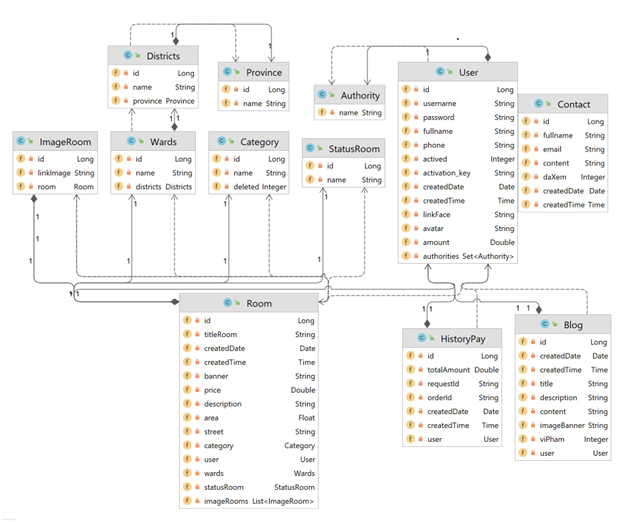
\includegraphics[width=\textwidth]{Figure/Picture7.png}
    \caption{Relationship}
    \label{fig:relationship}
\end{figure}

\section{Use cases diagram}

The use case diagram illustrates specific goals and how users interact with the system.
The ellipses within the system boundary represent the system's use cases or functions, while the stick figures symbolize the actors or users of the system.
The lines connecting the actors to the use cases indicate that the actors can perform those functions within the system to achieve their objectives.

\subsection{Use case general}

The website system comprises three main agents:
\subsubsection{Renter (or Tenant)}

Description: A user who directly interacts with the website's features such as viewing posts, searching for rental rooms, and accessing detailed room information.

Functions: View posts, search for rooms, view room details.

\subsubsection{Landlord}
Description: The user who posts room listings, with functions including managing posts, creating listings, depositing funds, logging in, and registering.

Functions: Manage posts, create listings, deposit funds, log in, register.

\subsubsection{Administrator}

Description: The role responsible for overseeing the entire system, including user management, post management, room category management, article management, and revenue management.

Functions: Manage users, manage posts, manage room categories, manage articles, manage revenue.

\subsection{Use case specifications}

\begin{enumerate}
    \item bruh
\end{enumerate}

\end{document}
